%
\hsection{Weak Entities}%
\label{sec:weakEntities}%
%
In the previous section, we made some big strides towards properly modelling people in our teaching management platform.
A particularly interesting aspect was the modeling of the different types of IDs and communication monikers.
Unifying IDs by using the new entity type \emph{ID Type} was a nice idea and we are pleased with ourselves.
Then we revisit our new \pgls{ERD} in \cref{fig:erdPerson2}.

And we remember something:
\emph{Relationship types do not have key attributes. Relationships are identified by the primary keys of the participating entities.}
Which entities are participating in our \emph{Has ID} relationship?
The \emph{Person} entities, identified by their surrogate key and the \emph{ID Type} entities, identified by their name.
If we apply the above rule, then this means that, actually, each person can only have one ID of any given type.
One mobile phone number.
One passport number.
One email address.

In other words:
We were happy too early.
Passports and visa expire and it is very possible that foreign members of our uni, during their stay, will have multiple different ones.
We did not yet solve the problem completely.

At least, we did not solve it well in terms of the conceptual model.
If we were to technically implement this model as a \postgresql\ \db, we could probably realize it in the way we \inQuotes{meant} it without too much of a hassle by using multiple tables and foreign keys and such and such.
But we want to do this properly also on a conceptual level.
Because the conceptual schema is a definition of the data that will go into our \db.
It should be correct.
The logical model that we design later must not diverge from the conceptual model.
This would eventually result in a pure nightmare for maintenance.
Luckily, the solution for this problem can be found in the different classes of entity types~\cite{S2024D:CDMERDE}.%
%
\begin{definition}[Strong Entity]%
A \emph{strong entity} exists independently of the other entities and has an own primary key.%
\end{definition}%
%
So far, we have modeled all of our data as strong entities.
However, there are also weak entities~\cite{P2006CITRD:CERDTRM,SS2005EIDDDFDB:CDDICAMP,S2024D:CDMERDE}.%
%
\begin{definition}[Weak Entity]%
A \emph{weak entity} is only identifiable by its attribute values \emph{and} the primary key(s) of one~(or multiple) entities.%
\end{definition}%
%
A \emph{weak entity} cannot exist on its own.
Its existence depends on at least one other entity, which is called its \emph{owner}.
It does not have an own primary key.
It has a partial key, i.e., a set of attributes that, combined with the primary keys of its owner(s), can be used to identify it in its entity set.%
%
\begin{definition}[Identifying Relationship]%
\label{def:identiRelation}%
An \emph{identifying relationship} links a strong entity to a weak entity and is required for identifying the weak entity.%
\end{definition}%
%
In an \pgls{ERD}, strong entities are symbolized by rectangles.
So far, we only modeled strong entities.
Weak entities are represented by double-lined rectangles.
The identifying relationships that connect them to other entities are symbolized by double-lined diamonds.
(Actually, we are talking here about entity types and relationship types, but writing this makes the text much harder to read\dots)

\begin{figure}%
\centering%
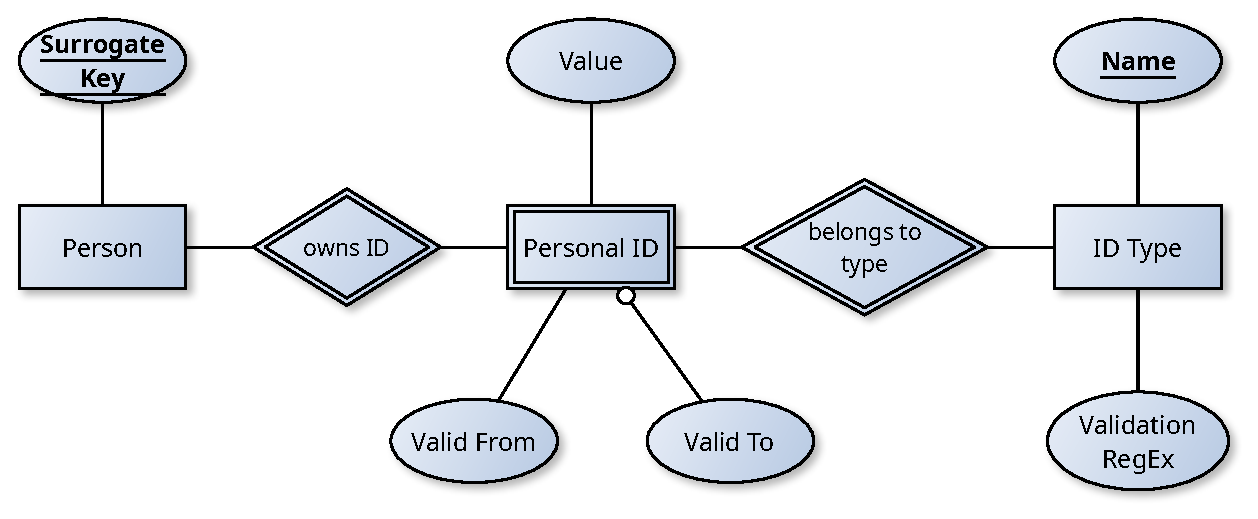
\includegraphics[scale=0.6]{\currentDir/erdPerson3}%
\caption{An improvement of \cref{fig:erdPerson2}: We now use weak entities to represent the ID values of a person.}%
\label{fig:erdPerson3}%
\end{figure}%
%
If we look at our \inQuotes{ID problem} again, we could model the \emph{has ID} relationship as a weak entity.
The weak entity would be identified by its own attribute values together with the primary key of the corresponding \emph{Person} entity and the primary key of the corresponding \emph{ID type} entity.
It would be a weak entity depending on two strong entities.

\Cref{fig:erdPerson3} illustrated this new situation.
The new weak entity is called \emph{Personal ID}.
It has the same attributes as the relationship in \cref{fig:erdPerson2}.
It is linked with identifying relationships to both the \emph{Person} and the \emph{ID Type} entities.
Each \emph{Personal ID}~entity is uniquely identified by its attributes \emph{Value}, \emph{Valid From}, and \emph{Valid To}~(which form the partial key) together with the primary keys \emph{Surrogate Key} of the \emph{Person} entity and \emph{Name} of the \emph{ID Type} entity.
Now a person can have multiple phone numbers, provided that they are different or valid at different time ranges.
A person can have different visa, because they will usually have different visa numbers.
Now we indeed have unified communication-based IDs such as mobile phone numbers, email addresses, \pgls{wechat} IDs together with document-based IDs such as, well, actual government issued IDs, visas, work permits, driver's licenses, etc.
And we can create new forms of ID if need be.%
%
\begin{definition}[Associative Entity]%
An \emph{associative entity}~(type) is an entity~(type) that has attributes and a primary key, but also serves as relationship that can link entities together.%
\end{definition}%
%
In an \pgls{ERD}, an associative entity is symbolized by a rectangle with a diamond inside.
They are mainly used to normalize and simplify many-to-many relationships.
They usually connect entities that have multiple interactions with each other.
However, we skip them here, as I see them more as an intermediate step when mapping entity models to \pgls{rdb} models.
At this stage, however, we do not want to concern ourselves with the relational \db\ structure~(yet).
It instead is our goal to more freely model the data structures that we will have to deal with~(and, hence implement) in our teaching management platform.

Be that as it may, we again made an important step forward.
By using weak entities, we can now cleanly model one-to-many and many-to-many relationships.
As example for this, we had the \inQuotes{has ID} relationship.
By using a weak entity type to replace this relationship, a person can have multiple IDs of the same type.
Since we also model email addresses and mobile phone numbers as IDs, that is an important feature.
Other candidates for using weak entities would be the relationships between professors, students, and modules.
This would allow us to model a situation where a student enrolls into the same module taught by the same professor in different semesters more cleanly.%
\FloatBarrier%
\endhsection%
%
